\documentclass{beamer}
\usepackage{hyperref}
\usepackage[T1]{fontenc}

% other packages
\usepackage{latexsym,amsmath,xcolor,multicol,booktabs,calligra}
\usepackage{graphicx,pstricks,listings,stackengine}

% dummy text; remove it when working on this template
\usepackage{lipsum}


\author{Ayush Raina}
\title{Maths Behind Denoising Diffusion Probabilistic Models (DDPM's) $\mathbb{I}$}
\institute{
    Indian Institute of Science \\
}
\date{\today}
\usepackage{Ritsumeikan} 


% defs
\def\cmd#1{\texttt{\color{red}\footnotesize $\backslash$#1}}
\def\env#1{\texttt{\color{blue}\footnotesize #1}}
\definecolor{deepblue}{rgb}{0,0,0.5}
\definecolor{deepred}{RGB}{153,0,0}
\definecolor{deepgreen}{rgb}{0,0.5,0}
\definecolor{halfgray}{gray}{0.55}

\lstset{
    basicstyle=\ttfamily\small,
    keywordstyle=\bfseries\color{deepblue},
    emphstyle=\ttfamily\color{deepred},    % Custom highlighting style
    stringstyle=\color{deepgreen},
    numbers=left,
    numberstyle=\small\color{halfgray},
    rulesepcolor=\color{red!20!green!20!blue!20},
    frame=shadowbox,
}

\begin{document}

\begin{frame}
    \titlepage
\end{frame}
    
\section*{Background}

\begin{frame}{ELBO - Evidance Lower Bound}
    \begin{enumerate}
        \item Evidence - Log Likelihood of observed data - $log (p(x))$ where $x \in \mathbb{R}^d$
        \item Evidance Lower Bound (ELBO) - Lower bound on the log likelihood of observed data - $log(p(x)) \geq ELBO$
    \end{enumerate}

    \[ \boxed{ELBO = \mathbb{E}_{q(z|x)}[log(\frac{p(x,z)}{q(z|x)})]} \]
    So let us see why ELBO is a lower bound on the log likelihood of observed data.
\end{frame}

\begin{frame}{Proof 1}
    We start with \( \log(p(x)) \), where \( z \) is the latent variable:

    \begin{align*}
        \log(p(x)) &= \log\left(\sum_z p(x, z)\right) && \text{(starting point)} \\
        &= \log\left(\sum_z \frac{p(x, z)}{q(z \mid x)} q(z \mid x)\right) && \text{(multiply and divide by \( q(z \mid x) \))} \\
        &= \log\left(\mathbb{E}_{q(z \mid x)}\left[\frac{p(x, z)}{q(z \mid x)}\right]\right) \\
        &\geq \mathbb{E}_{q(z \mid x)}\left[\log\left(\frac{p(x, z)}{q(z \mid x)}\right)\right] && \text{(Jensen's inequality)} \\
    \end{align*}

    We can use Jensen inequality because \( \log \) is a concave function.
\end{frame}

\begin{frame}{Proof 2}
    \begin{align*}
        \log(p(x)) &= \log(p(x)) \left( \sum_z q(z | x) \right) && \text{(starting point)} \\
        &= \sum_z q(z | x) \log(p(x)) && \text{} \\
        &= \mathbb{E}_{q(z|x)} \log\left( p(x) \right) && \text{} \\
        &= \mathbb{E}_{q(z|x)} \log\left( \frac{p(x)p(z|x)}{p(z|x)} \right) && \text{} \\
        &= \mathbb{E}_{q(z|x)} \left[ \log\left( \frac{p(x,z)}{p(z|x)} \right) \right] && \text{} \\
    \end{align*}
\end{frame}

\begin{frame}{Proof 2 Continued}
    \begin{align*}
        &= \mathbb{E}_{q(z|x)} \left[ \log\left( \frac{p(x,z)}{\textcolor{red}{q}(z|x)} \frac{\textcolor{red}{q}(z|x)}{p(z|x)} \right) \right] && \text{} \\
        &= \mathbb{E}_{q(z|x)} \left[ \log\left( \frac{p(x,z)}{\textcolor{red}{q}(z|x)} \right) + \log\left( \frac{\textcolor{red}{q}(z|x)}{p(z|x)} \right) \right] && \text{} \\
        &= \mathbb{E}_{q(z|x)} \left[ \log\left( \frac{p(x,z)}{\textcolor{red}{q}(z|x)} \right) \right] + \mathbb{E}_{q(z|x)} \left[ \log\left( \frac{\textcolor{red}{q}(z|x)}{p(z|x)} \right) \right] && \text{} \\
        &= ELBO + KL(\textcolor{red}{q}(z|x) || p(z|x)) && \text{} \\
    \end{align*}

    Since $KL(\textcolor{red}{q}(z|x) || p(z|x)) \geq 0$, we have $\log(p(x)) \geq ELBO$.
\end{frame}

\begin{frame}
    Now we know that 
    \[ \boxed{\log(p(x)) = \mathbb{E}_{q(z|x)} \left[ \log\left( \frac{p(x,z)}{q(z|x)} \right) \right] + KL(q(z|x) || p(z|x))} \]
    and due to the KL divergence term on the right hand side, we can say that ELBO is a lower bound on the log likelihood of observed data.
\end{frame}

\section*{VAE's}
\begin{frame}{Variational Autoencoder (VAE)}
    \begin{figure}
        \centering
        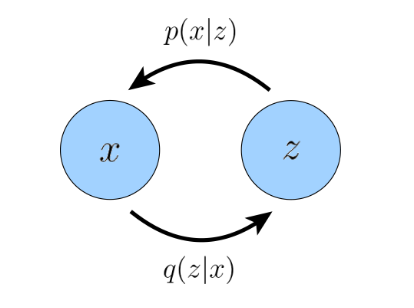
\includegraphics[width=0.4\textwidth]{Images/vae1.png}
        \caption{Variational Autoencoder}
    \end{figure}

    In default formulation in VAE paper, directly maximize ELBO using a \textcolor{blue}{variational} approach. \\

    We optimize for best possible $q_{\phi}(z|x)$ among family of posterior distributions which are parameterized by $\phi$.

\end{frame} 

\begin{frame}{Family of Posterior Distributions}
    The family of posterior distributions is generally choosen as multivariate gaussian with diagonal covariance matrix.

    \begin{align*}
        q_{\phi}(z|x) &= \mathcal{N}(z ; \mu_{\phi}(x), \sigma_{\phi}(x)) \\
        &= \mathcal{N}(z;\mu_{\phi}(x), diag(\sigma_{\phi}(x)))
    \end{align*}

    The prior is choosen as standard normal distribution 
    \begin{align*}
        p(z) &= \mathcal{N}(z;0, \mathbb{I}_{d \times d})
    \end{align*}
\end{frame}

\begin{frame}{Encoder and Decoder Network}
    When we maximize the ELBO, we are doing the following things to be specific:
    \begin{enumerate}
        \item Adjusting parameters $\phi$ in such a way that true latent distribution $p(z)$ is as close as possible to encoder outputs $p(z|x)$.
        \item Using these latents to regenerate the true data $x$ as close as possible.
    \end{enumerate}

    Let us see what they mean
\end{frame}

\begin{frame}{ELBO again}
    \begin{align*}
        ELBO &= \mathbb{E}_{q(z|x)}[log\left(\frac{p(x,z)}{q(z|x)}\right)] \\
        &= \mathbb{E}_{q(z|x)}[log \left( \frac{p(z)p(x | z)}{q(z|x)} \right)] \\
        &= \mathbb{E}_{q(z|x)}[log(p(x|z)) + log\left(\frac{p(z)}{q(z|x)}\right)] \\
        &= \mathbb{E}_{q(z|x)}[log(p(x|z))] + \mathbb{E}_{q(z|x)}[log\left(\frac{p(z)}{q(z|x)}\right)] \\
        &= \mathbb{E}_{q(z|x)}[log(p(x|z))] - \mathbb{E}_{q(z|x)}[log\left(\frac{q(z|x)}{p(z)}\right)] \\
        &= \mathbb{E}_{q(z|x)}[log(p(x|z))] - KL(q(z|x) || p(z))
    \end{align*}
\end{frame}

\begin{frame}{Continued}
    While maximizing ELBO, we did 2 things:
    \begin{enumerate}
        \item Maximize $\mathbb{E}_{q(z|x)}[log(p(x|z))]$ - This is the reconstruction term.
        \item Minimize $KL(q(z|x) || p(z))$ - This is the prior matching term.
    \end{enumerate}

    \bigskip

    Look at 2nd term first, this tries to bring $q(z|x)$ close to $p(z)$, which means given $x$, we are trying to model $z$ as close as possible to true latent distribution. 

    \bigskip

    Now look at 1st term in which we maximize the log likelihood of generating back the true $x$ from $z$. 
\end{frame}

\begin{frame}{Computing ELBO}
    There are 2 terms to be computed in ELBO:
    \begin{enumerate}
        \item Reconstruction term: $\mathbb{E}_{q(z|x)}[log(p(x|z))]$
    \end{enumerate}

    This can be estimated using sample averages. We sample $\{z^{(i)}\}_{i=1}^{N} \sim q(z|x)$  then above term can be computed as 
    \begin{align*}
        \mathbb{E}_{q(z|x)}[log(p(x|z))] &= \frac{1}{N} \sum_{i=1}^{N} log(p(x|z^{(i)}))
    \end{align*}
\end{frame}

\begin{frame}{Computing ELBO}
    \begin{enumerate}
        \setcounter{enumi}{1}
        \item KL Divergence term: $KL(q(z|x) || p(z))$
    \end{enumerate}
    Since both $q(z|x)$ and $p(z)$ are gaussian, there exists a closed form solution to compute KL divergence between 2 gaussians.
\end{frame}


\section*{MHVAE's}
\begin{frame}{Markovian Hierarchical Variational Autoencoder (MHVAE)}
    \begin{figure}
        \centering
        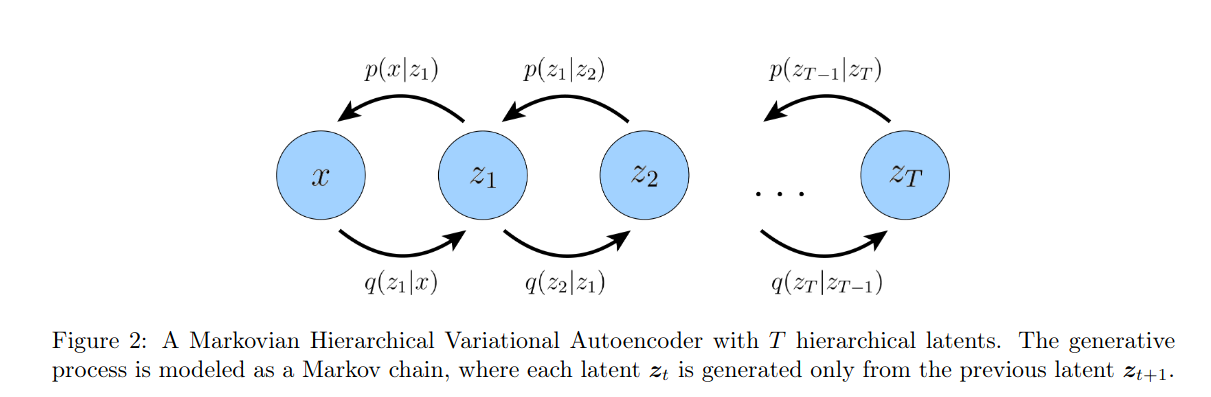
\includegraphics[width=1\textwidth]{Images/hvae1.png}
        \caption{Markovian Hierarchical Variational Autoencoder}
    \end{figure}

    In MHVAE, we have a hierarchical structure of latent variables. 
\end{frame}

\begin{frame}{Markovian Hierarchical Variational Autoencoder (MHVAE)}
    Now we have a hierarchical structure of latent variables.
    $z_1, z_2, \ldots, z_T$ are the latent variables at each time step. We can denote all these using $z_{1:T}$.
\end{frame}

\begin{frame}{Joint and Posterior}
    The Joint Distribution can be written as:  
    \begin{align*}
        p(x, z_{1:T}) &= p(z_T)p(x|z_1) \prod_{t=2}^{T} p(z_{t-1}|z_t)
    \end{align*}

    The posterior distribution can be written as:
    \begin{align*}
        p(z_{1:T}|x) &= \frac{p(x, z_{1:T})}{p(x)} \\
        &= \frac{p(x)p(z_1|x) \prod_{t=2}^{T} p(z_{t}|z_{t-1})}{p(x)} \\
        &= p(z_1|x) \prod_{t=2}^{T} p(z_{t}|z_{t-1}) \\
    \end{align*}
\end{frame}

\begin{frame}{Extending ELBO}
    \begin{align*}
        \log(p(x)) &= \log \left( \int p(x, z_{1:T}) dz_{1:T} \right) \\
        &= \log \left( \int p(x, z_{1:T}) \frac{q(z_{1:T}|x)}{q(z_{1:T}|x)} dz_{1:T} \right) \\
        &= \log \left( \mathbb{E}_{q(z_{1:T}|x)} \left[ \frac{p(x, z_{1:T})}{q(z_{1:T}|x)} \right] \right) \\
        &\geq \mathbb{E}_{q(z_{1:T}|x)} \left[ \log \left( \frac{p(x, z_{1:T})}{q(z_{1:T}|x)} \right) \right] && \text{(Jensen's Inequality)} \\
    \end{align*}
\end{frame}

\begin{frame}{Extending ELBO}
    \begin{align*}
        \log(p(x)) &\geq \mathbb{E}_{q(z_{1:T}|x)} \left[ \log \left( \frac{p(x, z_{1:T})}{q(z_{1:T}|x)} \right) \right] \\
        &= \mathbb{E}_{q(z_{1:T}|x)} \left[ \log \left( \frac{p(z_T)p(x|z_1) \prod_{t=2}^{T} p(z_{t-1}|z_t)}{q(z_{1:T}|x)} \right) \right] \\
        &= \mathbb{E}_{q(z_{1:T}|x)} \left[ \log \left( \frac{p(z_T)p(x|z_1) \prod_{t=2}^{T} p(z_{t-1}|z_t)}{q(z_1|x) \prod_{t=2}^{T} q(z_t|z_{t-1})} \right) \right] \\
    \end{align*}

    We will see how this expression can be broken down into terms that we have seen in VAE.
\end{frame}
\section*{VDM's}
\begin{frame}{Variational Diffusion Models (VDM's)}
    Variational Diffusion Model (VDM) is simply a MHVAE with 3 restrictions:
    \begin{enumerate}
        \item The dimension of latent variables is equal to dimension of data.
        \item Distribution of latent variables at each time step is Gaussian Centered at latent variable at previous time step. (This is not learnt, but fixed)
        \item Encoding transitions are done in such a way that distribution of latent variable at last time step is standard Gaussian.
    \end{enumerate}

    Let us see what changes occur in MHVAE when these restrictions are applied to it.
\end{frame}

\begin{frame}{Variational Diffuion Models (VDM's)}
    \begin{figure}
        \centering
        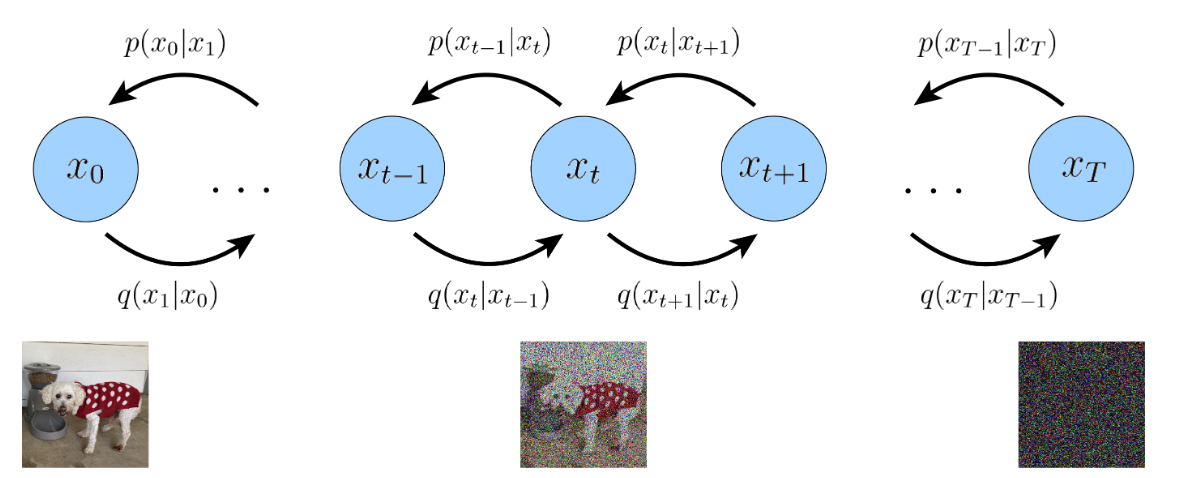
\includegraphics[width=1\textwidth]{Images/vdm1.png}
        \caption{Variational Diffusion Model}
    \end{figure}
\end{frame}

\begin{frame}{Variational Diffusion Models (VDM's)}
    \begin{itemize}
        \item $x_0$ represents true data observations.
        \item $x_t$ represents intermediate noisy version of data.
        \item $x_T$ represents pure Gaussian noise.
    \end{itemize}
\end{frame}

\begin{frame}{Restriction 1}
    According to slight change of notation in previous slide, VDM's posterior is same as MHVAE's posterior which can now be written as:
    \begin{align*}
        q(x_{1:T}|x_0) &= \prod_{t=1}^{T} q(x_t|x_{t-1}) && \text{(VDM's Posterior)}
    \end{align*}
    instead of 
    \begin{align*}
        q(z_{1:T}|x) &= p(z_1|x) \prod_{t=2}^{T} q(z_t|z_{t-1}) && \text{(MHVAE's Posterior)}
    \end{align*}
\end{frame}

\begin{frame}{Restriction 2}
    Unlike MHVAE, distribution of latent variable at each time step is not learnt, but is fixed. Mathematically, the encoder transitions can be written as:
    \begin{align*}
        q(x_t|x_{t-1}) &= \mathcal{N}(x_t; \sqrt{\alpha_t}x_{t-1}, (1-\alpha_t) \mathbb{I}_{d \times d}) 
    \end{align*}

    Distribution of latent variable $x_t$ at each time step is gaussian centered at latent variable at previous time step $x_{t-1}$.
\end{frame}

\begin{frame}{Restriction 3}
    Gaussian Transitions are made in such a way that distribution of final latent variable $x_T$ is standard Gaussian. Mathematically, this can be written as:
    \begin{align*}
        q(x_T|x_{T-1}) &= \mathcal{N}(x_T; 0, \mathbb{I}_{d \times d})
    \end{align*}

    Hence Joint Distribution of VDM can be written as:
    \begin{align*}
        p(x_{0:T}) &= p(x_T) \prod_{t=1}^{T} q(x_{t-1}|x_{t}) && p(x_T) \sim \mathcal{N}(0, \mathbb{I}_{d \times d})
    \end{align*}
    Instead of
    \begin{align*}
        p(x,z_{1:T}) &= p(x_T)p(x|z_1) \prod_{t=2}^{T} q(z_{t-1}|z_{t}) && \text{(MHVAE's Joint)}
    \end{align*}
\end{frame}

\begin{frame}{Learning conditionals}
    Since encoder transitions are fixed for each time steps, we are only interested in learning conditionals $p(x_{t-1}|x_t)$ so that we can simulate new data. 

    \bigskip

    We can achieve this by maximizing ELBO for VDM. To show that maximizing ELBO actually helps in learning conditionals, we will first split ELBO in different components like we did in VAE and got the reconstruction term and prior matching term.
\end{frame}

\begin{frame}{Breaking down ELBO}
    We know that ELBO for MHVAE can be written as:
    \begin{align*}
        ELBO &=  \mathbb{E}_{q(z_{1:T}|x)} \left[ \log \left( \frac{p(x, z_{1:T})}{q(z_{1:T}|x)} \right) \right] \\
    \end{align*}
    According to notation's for VDM, we can write ELBO as:
    \begin{align*}
        ELBO &=  \mathbb{E}_{q(x_{1:T}|x_0)} \left[ \log \left( \frac{p(x_{0:T})}{q(x_{1:T}|x_0)} \right) \right] \\
    \end{align*}
\end{frame}

\begin{frame}{Breaking down ELBO}
    We further saw that ELBO for MHVAE can be written as:
    \begin{align*}
        ELBO &= &= \mathbb{E}_{q(z_{1:T}|x)} \left[ \log \left( \frac{p(z_T)p(x|z_1) \prod_{t=2}^{T} p(z_{t-1}|z_t)}{q(z_1|x) \prod_{t=2}^{T} q(z_t|z_{t-1})} \right) \right] \\
    \end{align*}

    In our case we can write this as:
    \begin{align*}
        ELBO &= \mathbb{E}_{q(x_{1:T}|x_0)} \left[ \log \left( \frac{p(x_T) \prod_{t=1}^{T} p(x_{t-1}|x_t)}{\prod_{t=1}^{T} q(x_t|x_{t-1})} \right) \right] \\
    \end{align*}

    Let us now further simplify this expression.
\end{frame}

\begin{frame}{Breaking down ELBO}
    \begin{align*}
        ELBO &= \mathbb{E}_{q(x_{1:T}|x_0)} \left[ \log \left( \frac{p(x_T) \prod_{t=1}^{T} p(x_{t-1}|x_t)}{\prod_{t=1}^{T} q(x_t|x_{t-1})} \right) \right] \\
        &= \mathbb{E}_{q(x_{1:T}|x_0)} \left[ \log \left( \frac{p(x_T)p(x_0|x_1) \prod_{t=2}^{T} p(x_{t-1}|x_t)}{\prod_{t=1}^{T} q(x_t|x_{t-1})} \right) \right] \\
        &= \mathbb{E}_{q(x_{1:T}|x_0)} \left[ \log \left( \frac{p(x_T)p(x_0|x_1) \prod_{t=2}^{T} p(x_{t-1}|x_t)}{q(x_T|x_{T-1}) \prod_{t=1}^{T-1} q(x_t|x_{t-1})} \right) \right] \\
        &= \mathbb{E}_{q(x_{1:T}|x_0)} \left[ \log \left( \frac{p(x_T)p(x_0|x_1) \prod_{t=1}^{T-1} p(x_{t}|x_{t+1})}{q(x_T|x_{T-1}) \prod_{t=1}^{T-1} q(x_t|x_{t-1})} \right) \right] \\
    \end{align*}
\end{frame}

\begin{frame}{Breaking down ELBO}
    \begin{align*}
        &= \mathbb{E}_{q(x_{1:T}|x_0)} \left[ \log \left( \frac{p(x_T)p(x_0|x_1)}{q(x_T|x_{T-1})} \right) + \sum_{t=1}^{T-1} \log \left( \frac{p(x_{t}|x_{t+1})}{q(x_t|x_{t-1})} \right) \right] \\
        &= \mathbb{E}_{q(x_{1:T}|x_0)} \left[ \log \left( \frac{p(x_T)p(x_0|x_1)}{q(x_T|x_{T-1})} \right) \right] + \sum_{t=1}^{T-1} \mathbb{E}_{q(x_{1:T}|x_0)} \left[ \log \left( \frac{p(x_{t}|x_{t+1})}{q(x_t|x_{t-1})} \right) \right] \\
    \end{align*}

    First Term can further be simplified into
    \begin{align*}
        &= \mathbb{E}_{q(x_{1:T}|x_0)} \left[ \log \left( \frac{p(x_T)}{q(x_T|x_{T-1})} \right) \right] + \mathbb{E}_{q(x_{1:T}|x_0)} \left[ \log \left( p(x_0|x_1) \right) \right] \\
    \end{align*}
\end{frame}

\begin{frame}{Reconstruction Term}
    We got 3 terms:
    \begin{enumerate}
        \item $\mathbb{E}_{q(x_{1:T}|x_0)} \left[ \log \left( p(x_0|x_1) \right) \right]$
    \end{enumerate}
    \bigskip
    Since inside expression is independent of $x_{2:T}$, we can write this as:
    \begin{align*}
        &= \mathbb{E}_{q(x_{1}|x_0)} \left[ \log \left( p(x_0|x_1) \right) \right] && \text{(\textcolor{red}{reconstruction term})}
    \end{align*}

    maximizing ELBO results in maximizing this term which is log likelihood of getting back original data sample from latent variable at first time step.
\end{frame}

\begin{frame}{Prior Matching Term}
    \begin{enumerate}
        \setcounter{enumi}{1}   
        \item $\mathbb{E}_{q(x_{1:T}|x_0)} \left[ \log \left( \frac{p(x_T)}{q(x_T|x_{T-1})} \right) \right]$
    \end{enumerate}
    We can simplify this expression as follows:
    \begin{align*}
        &= \mathbb{E}_{q(x_{T-1,T}|x_{0})} \left[ \log \left( \frac{p(x_T)}{q(x_T|x_{T-1})} \right) \right] \\
        &= \int q(x_{T-1,T}|x_{0}) \log \left( \frac{p(x_T)}{q(x_T|x_{T-1})} \right) dx_{T-1} dx_T \\
        &= \int q(x_{T-1}|x_{0}) \left[ q(x_T|x_{T-1}) \log \left( \frac{p(x_T)}{q(x_T|x_{T-1})} \right) dx_T \right] dx_{T-1} \\
        &= -\int q(x_{T-1}|x_{0}) D_{KL} \left( q(x_T|x_{T-1}) || p(x_T) \right) dx_{T-1} \\
        &= -\mathbb{E}_{q(x_{T-1}|x_{0})} \left[ D_{KL} \left( q(x_T|x_{T-1}) || p(x_T) \right) \right] 
    \end{align*} 
\end{frame}

\begin{frame}{Prior Matching Term}
    \begin{align*}
        &= -\mathbb{E}_{q(x_{T-1}|x_{0})} \left[ D_{KL} \left( q(x_T|x_{T-1}) || p(x_T) \right) \right] 
    \end{align*} 

    This is \textcolor{red}{prior matching term}, maximizing ELBO results in minimizing this term, which forces the distribution of latent variable at last time as close as possible to $p(x_T) \sim \mathcal{N}(0, \mathbb{I}_{d \times d})$.
\end{frame}

\begin{frame}{Consistency Term}
    \begin{enumerate}
        \setcounter{enumi}{2}
        \item $\mathbb{E}_{q(x_{1:T}|x_0)} \left[ \log \left( \frac{p(x_{t}|x_{t+1})}{q(x_t|x_{t-1})} \right) \right]$
    \end{enumerate}

    This term can be simplified as:
    \begin{align*}
        &= \mathbb{E}_{q(x_{t-1,t,t+1}|x_{0})} \left[ \log \left( \frac{p(x_{t}|x_{t+1})}{q(x_t|x_{t-1})} \right) \right] \\
        &= \int q(x_{t-1,t,t+1}|x_{0}) \log \left( \frac{p(x_{t}|x_{t+1})}{q(x_t|x_{t-1})} \right) dx_{t-1} dx_t dx_{t+1} \\
        &= \int q(x_{t+1}|x_{0}) q(x_{t-1}|x_{t+1}) \left[ q(x_{t}|x_{t-1}) \log \left( \frac{p(x_{t}|x_{t+1})}{q(x_t|x_{t-1})} \right) dx_t \right] dx_{t-1,t+1} \\
        &= -\int q(x_{t+1}|x_{0}) q(x_{t-1}|x_{t+1}) D_{KL} \left( q(x_t|x_{t-1}) || p(x_t|x_{t+1}) \right) dx_{t-1,t+1} \\
        &= -\mathbb{E}_{q(x_{t+1}|x_{0}) q(x_{t-1}|x_{t+1})} \left[ D_{KL} \left( q(x_t|x_{t-1}) || p(x_t|x_{t+1}) \right) \right]
    \end{align*}
\end{frame}

\begin{frame}{Consistency Term}
    \begin{align*}
        &= -\mathbb{E}_{q(x_{t-1,t+1}|x_{0})} \left[ D_{KL} \left( q(x_t|x_{t-1}) || p(x_t|x_{t+1}) \right) \right]
    \end{align*}

    This is \textcolor{red}{consistency term}, maximizing ELBO results in minimizing this term, which ensures that distribution of noised image at time step $t$ i.e $q(x_t|x_{t-1})$ is as close as possible to distribution of denoised image at time step $t$ i.e $p(x_t|x_{t+1})$.
    
\end{frame}

\begin{frame}{ELBO}
    Finally we saw that ELBO = reconstruction term + prior matching term + consistency term where:
    \begin{enumerate}
        \item Reconstruction term $\mathbb{E}_{q(x_{1}|x_0)} \left[ \log \left( p(x_0|x_1) \right) \right]$
        \item Prior Matching term $-\mathbb{E}_{q(x_{T-1}|x_{0})} \left[ D_{KL} \left( q(x_T|x_{T-1}) || p(x_T) \right) \right]$
        \item Consistency term $-\mathbb{E}_{q(x_{t-1,t+1}|x_{0})} \left[ D_{KL} \left( q(x_t|x_{t-1}) || p(x_t|x_{t+1}) \right) \right]$
    \end{enumerate}
    \bigskip
    \textcolor{red}{maximizing ELBO results in minimizing prior matching term and consistency term and maximizing reconstruction term.}
\end{frame}

% thank you slide
\begin{frame}{Thank You!}
    \begin{center}
        \Huge Thank You!
    \end{center}
\end{frame}

%References
\begin{frame}{References}
    \begin{enumerate}
        \item Understanding Diffusion Models: A Unified Perspective
    \end{enumerate}
\end{frame}

\end{document}

